\chapter{\texttt{ObjectDetector} node}

\section{Description}
	Once we have some initial knowledge on CNNs applied to image processing, thank to the \texttt{DigitClassifier} component, we develop a new deep learning component, \texttt{ObjectDetector}, which is capable of \emph{detect objects in a real-time image stream}\footnote{For a better compatibility with future usages for this component, it is able to process images from a local video/webcam directly using OpenCV (so \texttt{comm} is not required for the execution), specifying this in the YML configuration file.}.\\

	This component has a generic functionality, as the real-time processing capability is only used to display on the image where the objects are, wrapping them on what is called \emph{bounding boxes}. These boxes are the rectangles inside of which, theoretically the detected object is contained, and are delivered along the \emph{detection score}, and the corresponding \emph{class} detected. We will go further on this later.\\
	\begin{figure}[h]
		\centering
		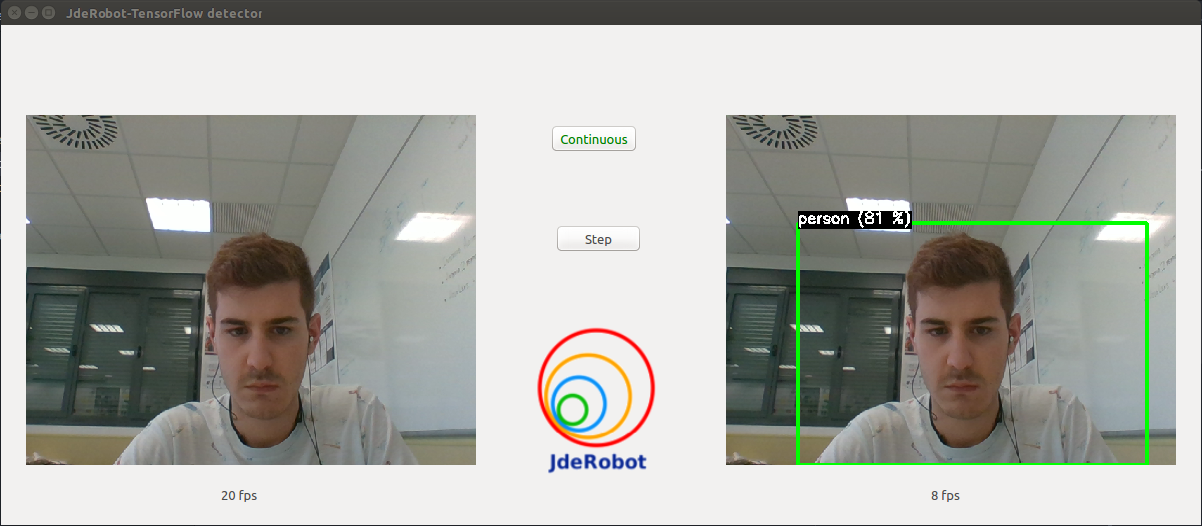
\includegraphics[width=4in]{images/objectdetector}
		\caption{\texttt{ObjectDetector} working.}
		\label{fig:5_objectdetector}
	\end{figure}
	
	We can notice that the type of problem that we are trying to solve now is different. Until now, we were trying to \emph{classify} images, based on a certain features that the network extracted by itself (the response always a classification, inferring an output even when no digit was shown to the camera, like shown on \autoref{fig:5_classifier_not_detecting}). Now, we are focused on \emph{detecting} objects inside an image. In other words, we want to distinguish whether an object (of a specific class or type) is present or not in the image that is being currently seen.
	
	\begin{figure}
		\centering
		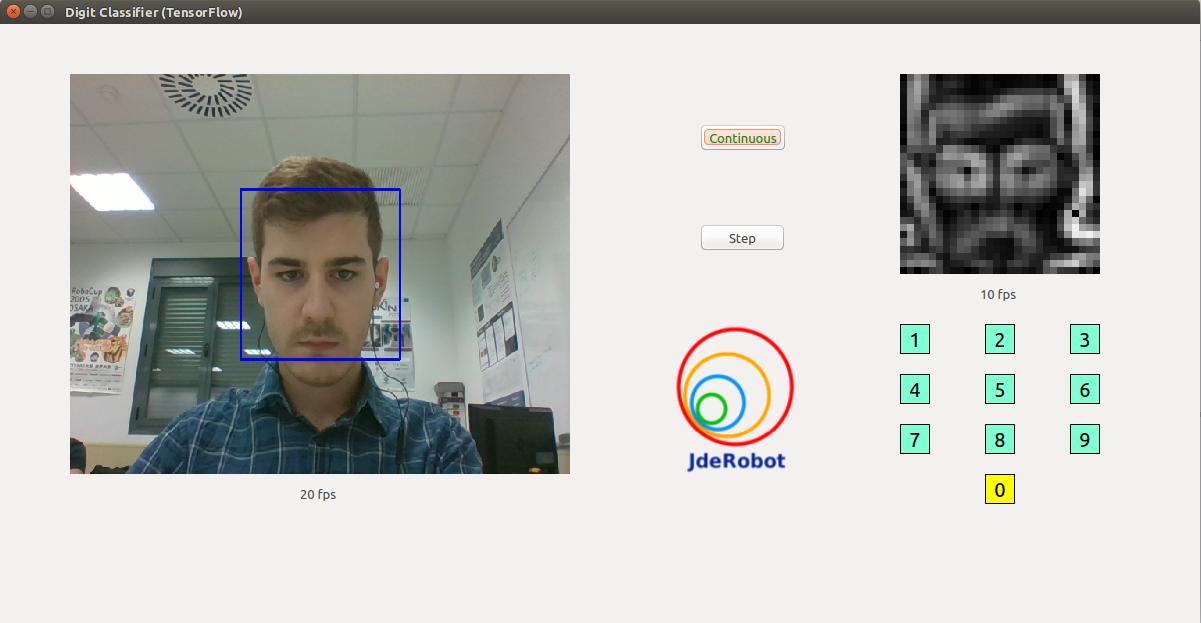
\includegraphics[width=4in]{images/digitclassifier_not_detection}
		\caption{\texttt{DigitClassifier}: a digit was always returned (or a subtle way of a computer to call you waste of space).}
		\label{fig:5_classifier_not_detecting}
	\end{figure}
	
	
	It should be mentioned that this purpose requires a much more complex CNN, which leads to a significantly heavier computational load on the machine (and, as a consequence, an importantly bigger inference time). Hence, a GPU-version of TensorFlow is highly recommended, as the CPU-version would take way too long for a real-time operation system.\\
	
	Due to this mentioned complexity, \emph{training a detection CNN} is out of the scope of this project (even so, with the proper resources, we could do it with some open-access labeled image datasets). Instead of this, we will pick some public models that the TensorFlow team has made available on the \emph{Detection Model Zoo}\footnote{\url{https://github.com/tensorflow/models/blob/master/research/object_detection/g3doc/detection_model_zoo.md}} (\autoref{fig:5_model_zoo}). On a parallel way, we have created a public mirror repository%
	\footnote{\url{http://jderobot.org/store/deeplearning-networks/}} inside JdeRobot containing some useful found models (for TensorFlow and Keras respectively).\\
	
	\begin{figure}[h]
		\centering
		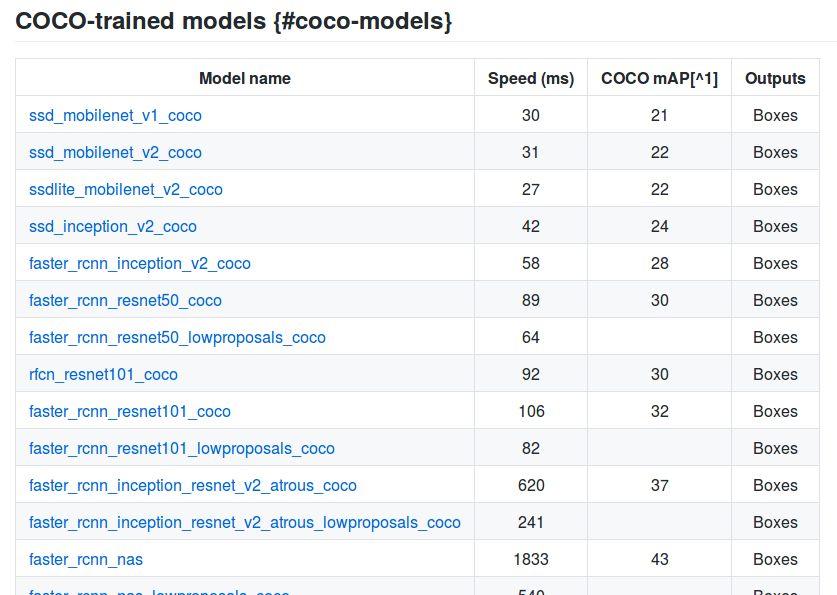
\includegraphics[width=4.5in]{images/detection_model_zoo}
		\caption{Some available models (July 2018) with their respective performance indicators.}
		\label{fig:5_model_zoo}
	\end{figure}
	
	
	These models have been trained on first-tier hardware, and are materialized in serialized files containing the graph structure and the corresponding weights for each neuron, on a ProtoBuf format (as we stated on \autoref{sec:3_tensorflow}). These model files are \textit{loadable at runtime} on a TensorFlow graph instance, so invoking one of these imported graphs is an easy task:
	\begin{figure}[h]
		\begin{lstlisting}
detection_graph = tf.Graph() # New graph instance.

# We use a context generator to set this graph as the default one
# on the TF backend:
with detection_graph.as_default():
	graph_def = tf.GraphDef()
	graph_def.ParseFromString(model_file)
	# We load this definition into the backend
	# (which contains the Graph instance).
	tf.import_graph_def(graph_def)
	
		\end{lstlisting}
		\caption{Generic model loading process.}
		\label{fig:5_load_model}
	\end{figure}

	
This way, we have successfully loaded the graph with its weights on the TensorFlow backend. The Python class (\texttt{DetectionNetwork}) we have defined allows to do this, choosing the desired model and dataset\footnote{Compatible with COCO, Kitti, OID and Pascal VOC datasets.} (we don't want the network to label a person as a dog) through the global YML configuration file.\\

Another thing to mention is the fact that, defining a \texttt{Writer} on the load process, we can inspect the graph structure on TensorBoard, as we will do later.

\section{Node architecture}
	\label{sec:5_node_architecture}
	\begin{figure}[h]
		\centering
		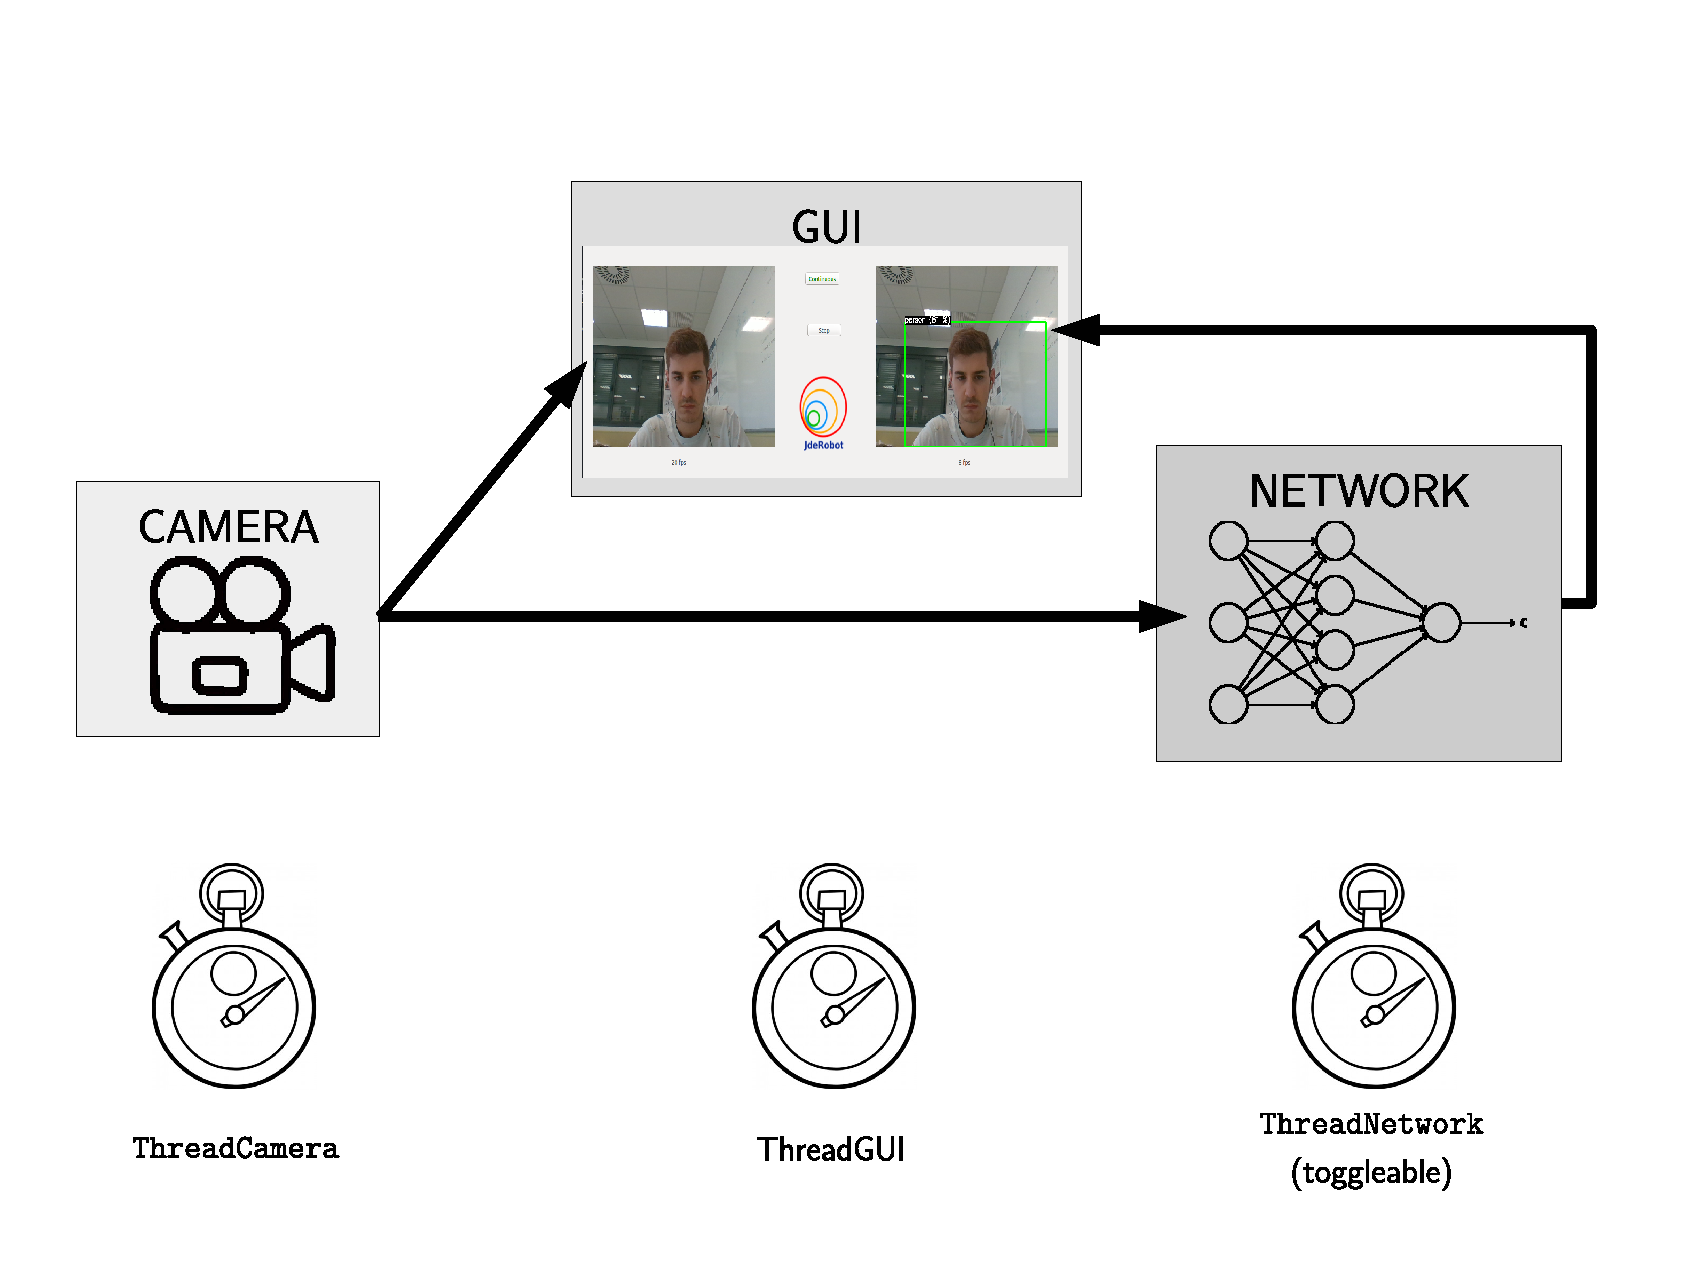
\includegraphics[width=4.5in]{images/objectdetector_infrastructure}
		\caption{Infrastructure of the component (3 threads).}
	\end{figure}
	
	This node inherits the architecture developed for the \emph{classification node}, consisting on 3 parallel threads. These threads drive the behavioral of separated objects, committed to perform independent tasks:
	\begin{itemize}
		\item \textit{Camera}: grabs the current image delivered by the communication framework (\texttt{comm} or OpenCV).
		
		\item \textit{GUI}: launches and updates the interface, with the fresh image from the camera. That image is drawn twice, as one of the representation (left) corresponds to the raw image from the camera, and the other one (right) is modified, including the bounding boxes, class and score for each detected object. This mentioned information is taken from the neural network. Hence, this component is connected respectively to the image source and the neural network.
		
		\item \textit{Network}: infers continuously the detected objects from the last received image, on an asynchronous way. When an inference is completed, the result (a set for each detection of bounding box, class and score for each single detection) is stored inside the \texttt{network} element. When the GUI needs the latest inference data, it just takes that data without any blocking call nor interrupting any process. This complies with the stated asynchronism requirement. 
	\end{itemize}
	
	Given this pretty identical structure to the \texttt{DigitClassifier} node, the schematic code to instantiate the program is the same than \texttt{DigitClassifier}'s (\autoref{fig:4_digitclassifier_code}).

	
\section{Detection CNN: SSD}
	As we have just mentioned, our application uses a SSD (\emph{Single Shot Multibox Detector}) CNN to perform the detection task. This choice has fundamentally taken based on the real-time performance expected from the component. We want it to make inferences as fast as possible (with a reasonable precision), so we chose this kind of architecture (it's more, it yields as good results as its slower counterparts).\\
	
	The high speed of inference of this kind of detectors is explained with the fact that \emph{it performs a single feed-forward pass} of the image through the network (on a \emph{single shot}, as it name states). According to its official release \cite{ssd-paper}, the rest of \emph{state-of-the-art} detection CNN technologies approach performing \emph{feature scaling} and \emph{bounding box proposals}. These techniques require more than one pass of the image or, at least, more than one single architecture, which rises the inference time.\\
	\subsection{Architecture}
		As we can observe in \autoref{fig:5_objectdetector_graph}, a \emph{SSD} detector has a defined network architecture, with some key aspects to keep its performance vs. inference time on the highest possible value. An inspection of the architecture using TensorBoard (\autoref{fig:5_objectdetector_graph}) reveals the pipeline structure, which is described below.
		
			
			\begin{figure}[h]
				\centering
				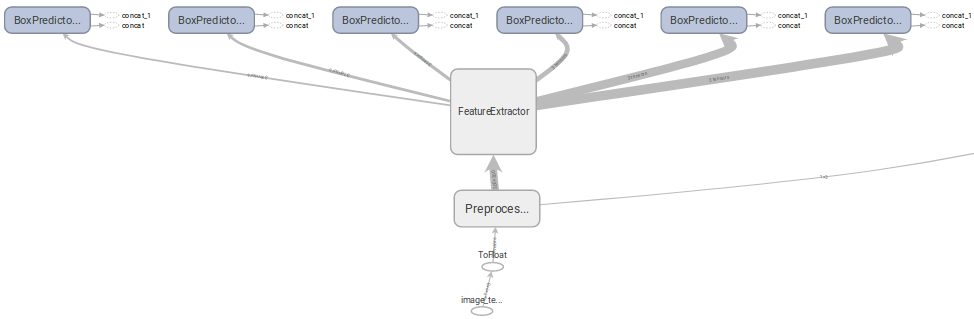
\includegraphics[width=\linewidth]{images/objectdetector_graph}
				\caption{SSD architecture on our model.}
				\label{fig:5_objectdetector_graph}
			\end{figure}
			

		\begin{enumerate}
			
			\item \emph{Preprocessing}: a first \emph{reshaping} stage is necessary due to the SSD operation. We can mention that this reshape is performed \emph{inside} the neural network, working directly with tensors on the GPU, which is probably faster than if we performed it with higher-level operations. This block reshapes the image to a 300$\times$300 size, which is the most typical image size on an SSD detector.
			\item \emph{Feature Extractor}: the architecture on a SSD CNN is based on a first group of layers (typically called the \emph{base network}), which deals with the \emph{feature extraction} part (as on the first stage of the classification network we designed on \autoref{sec:4_classif_cnn}). This particular model has a \emph{MobileNet} based feature extraction network\footnote{\emph{MobileNets} are originally designed to embed \emph{small, low latency} deep learning systems on low-spec devices \cite{mobilenet}, squeezing the trade-off between performance and inference time. So, we can reuse that part of its architecture for our proposal.}.  As it is formed by a concatenation of convolutional layers (\autoref{fig:5_mobilenet}), the resulting \emph{feature maps} will be gradually smaller and deeper while we go forward. These maps sets will be convolved with the original image, so the smaller the activation map is, the bigger its \emph{receptive field} will be (hence, it will useful to detect bigger objects). Given this, we are capable of \emph{extract} 6 intermediate sets (described on \autoref{tab:5_sets_imagenet}), with the objective of \emph{detect objects of different sizes}.
			
			\begin{figure}[h]
				\centering
				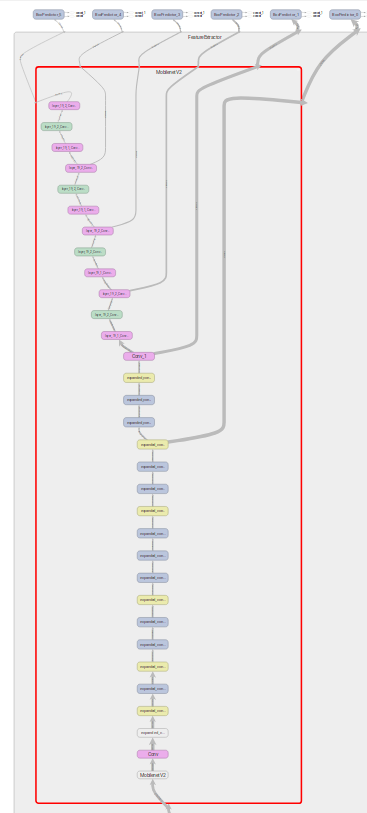
\includegraphics[width=2in]{images/ssd_mobilenet_2}
				\caption{\emph{MobileNet} pipeline.}
				\label{fig:5_mobilenet}
			\end{figure}

			\begin{table}[h]
				\centering
				\begin{tabular}{|c|c|c|}\hline
					\textbf{\# Set} & \textbf{Shape} & \textbf{Depth} \\ \hline
					1              & 1$\times$1     & 128            \\
					2              & 2$\times$2     & 256            \\
					3              & 3$\times$3     & 256            \\
					4              & 5$\times$5     & 512            \\
					5              & 10$\times$10   & 1280           \\
					6              & 19$\times$19   & 576           \\ \hline
				\end{tabular}
				\caption{Description of the 6 extracted feature maps sets on our implementation.}
				\label{tab:5_sets_imagenet}
			\end{table}
	
			
			\item \emph{Box Predictors}: later, for each extracted set, a dedicated operation is performed (that's the reason why we have 6 identical boxes on the TensorBoard analysis (\autoref{fig:5_objectdetector_graph}). They will perform the same operation but in patches of different sizes/depths, to detect \emph{objects on different scales}). Into this component, for each layer of the extracted feature set, a small set (3-4 typically) of bounding boxes (called \emph{priors}) with different \emph{aspect ratios} are generated (\autoref{fig:5_ssd_generated_boxes}).
			
			\begin{figure}[h]
				\centering
				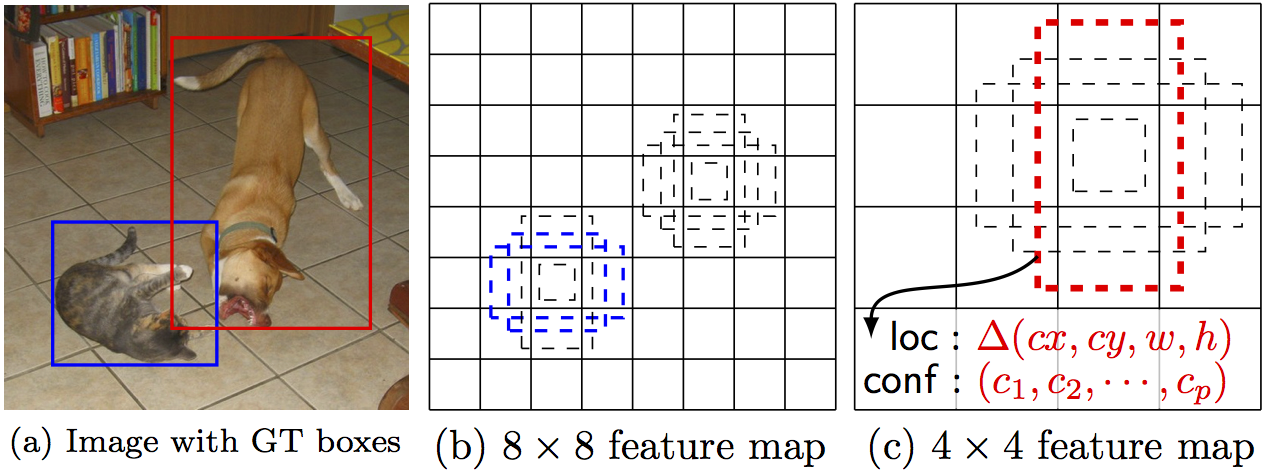
\includegraphics[width=3.5in]{images/ssd_generated_boxes}
				\caption{A set of boxes are generated centered on each point of every feature map \cite{ssd-paper}.}
				\label{fig:5_ssd_generated_boxes}
			\end{figure}
			
			After this, these \emph{priors} are convolved with small filters (one per depth channel), which outputs \emph{softmaxed confidence values for each known class}, and \emph{offsets/adjustments for the generated bounding box}. So, for each detected object (on that scale), we know the score for each class and its estimated position inside the feature map.
			
			\item \emph{Postprocessor}: this element does not appear in \autoref{fig:5_objectdetector_graph}, it had to be cropped on the image for geometrical reasons, but it is present on the network structure. It combines the output of all the 6 \emph{Box Predictors} (which contain detections for each feature map set), and applies a \emph{Non-Maximum Suppresor}, which only retains the most confident detections, and scales its position to the original image size.
		\end{enumerate}
	
	This way, we have a system that, for each introduced image, returns a collection of:
	\begin{itemize}
		\item \emph{Classes}: the detected class (person, cell phone, airplane, dog...) inferred.
		\item \emph{Scores}: the confidence $\in [0,1]$ the network has on each object belonging to the decided class (which was the most probable one while the detection was performed).
		\item \emph{Boxes}: the coordinates of the \emph{bounding box} which wraps the detected object, typically expressed as the coordinates of its top-left and bottom-right corners.
	\end{itemize}
	
	As this is suitable for real-time performance, we are now capable, on a standard computer hardware, to feed it with a video streaming (a file, or live camera images).
	
	\subsection{Importing a pretrained model}
		We have mentioned the training process of this kind of CNNs. It is not complicated from the point of view of the entire system (\emph{black box}), it only needs a dataset containing images with classes and \emph{ground truth boxes}\footnote{\emph{Ground truth}: what the network knows to trust, what is told it to be the true position of the object to detect.} (Microsoft's COCO, Pascal VOC, etc.). With these images, the SSD architecture learns to perform a better \emph{regression}, to achieve a better fitting of the boxes with respect to the original ones, evaluating it using the \emph{Jaccard similarity coefficient}, or IoU (\emph{Intersection over Union}). This measure evaluates how good the overlap between the true and the estimated boxes is (\autoref{fig:5_iou}). Additionally, it performs a standard \emph{back-propagation} process similar to the one we executed on the previous component (\autoref{sec:4_train}).
		
		\begin{figure}[h!]
			\centering
			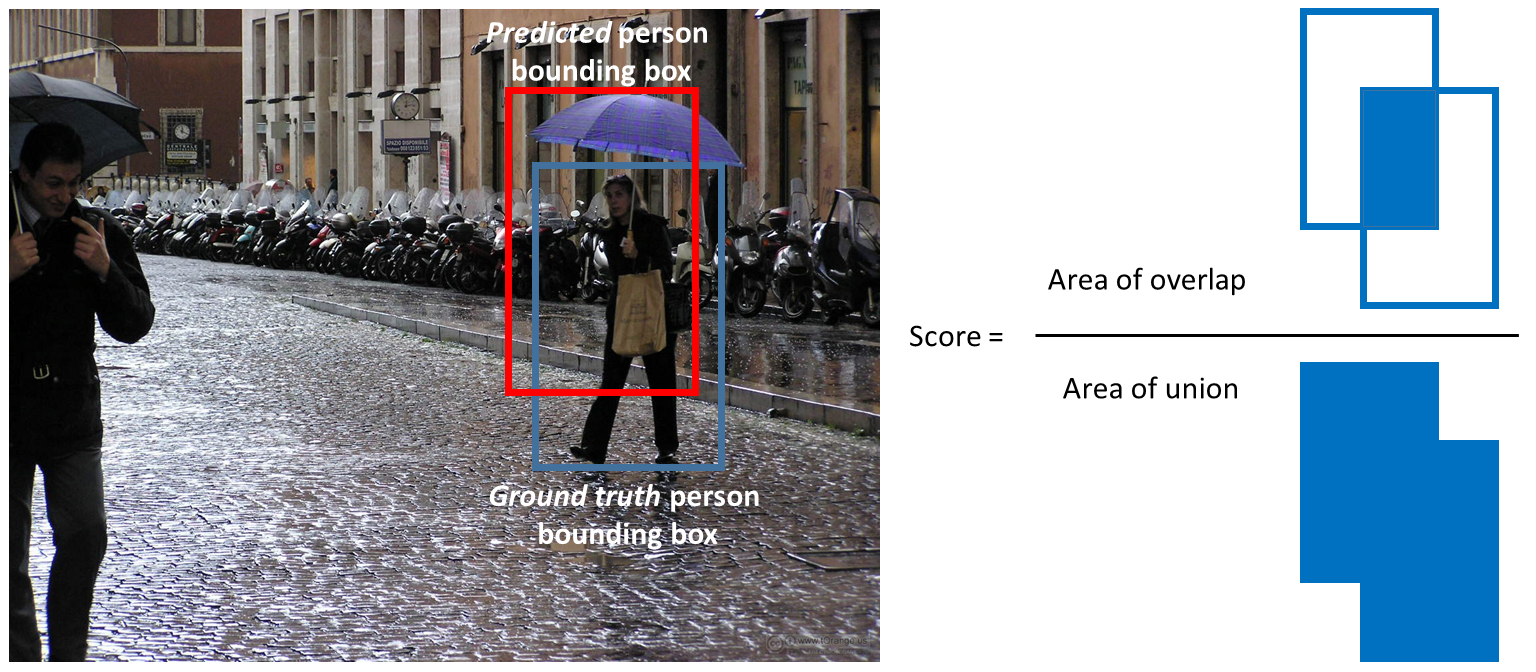
\includegraphics[width=3.7in]{images/detection_iou}
			\caption{\emph{Jaccard similarity coefficient} on a detection (performance indicator used for training a detector).}
			\label{fig:5_iou}
		\end{figure}
	
		The much heavier complexity of this task is not our point where to focus, so we will \emph{embed pretrained models}, available thank to the TensorFlow team on the previously mentioned \emph{Detection Model Zoo}\footnote{\url{https://github.com/tensorflow/models/blob/master/research/object_detection/g3doc/detection_model_zoo.md}}.\\
		
		In our case, we have selected a \emph{SSD detector}, with a \emph{MobileNet v2} feature extraction base network, trained on the \emph{COCO} dataset \footnote{\url{http://cocodataset.org}}. As this dataset support 90 object types (\emph{person, dog, airplane, toothbrush, apple, cellphone, etc.}, those are the classes we are able to detect. It provides a lightweight structure which performs inferences at a framerate of approximately 14 fps (on the currently available hardware).\\
		
		We load this network architecture and weights on the mentioned manner (\autoref{fig:5_load_model}). 
	
	
	\subsection{Network output}
		As we have specified, the detection network yields detected \emph{classes, scores} and \emph{bounding boxes}. Respecting the required asynchronous behavioral, this data is deposited on an accessible zone for the GUI, allowing to begin another iteration when requested.\\
		
		Therefore, as described at \autoref{sec:5_node_architecture} the GUI instance grabs the last detection data the network left on the shared placeholder, and draws it on the visible user interface (\autoref{fig:5_whole_pipeline}).
		
		\begin{figure}[h!]
			\centering
			\includegraphics[width=5in]{images/objectdetector_network_yield}
			\caption{Information flow through the whole pipeline.}
			\label{fig:5_whole_pipeline}
		\end{figure}

\vspace{3.5in}
\section{Experiment: testing different architectures}
	The implemented generic class (\texttt{DetectionNetwork}) allows to load on runtime a pretrained TensorFlow model of neural network. We can take advantage of this to perform a quantitative timing benchmark of different architectures and/or datasets, among the available models on the TensorFlow Detection Zoo\footnote{\url{https://github.com/tensorflow/models/blob/master/research/object_detection/g3doc/detection_model_zoo.md}}. As this node is a implementation on a real time video streaming, measures can't be taken on \emph{precision} terms. However, a deeper analysis of that kind can be performed with the JdeRobot tool \texttt{DetectionSuite} (described on \autoref{sec:dl_jderobot}), which allows to measure performance in terms of advanced markers, as \emph{Jaccard Index}, precision and recall.\\
	
	The timing tests (\autoref{tab:5_tests}) have been performed under the described available hardware, computing the mean inference time over 200 inferences on a people walking video (\autoref{fig:5_benchmark_screen}). Notice that the frame rate and/or resolution are not relevant, as every image experiments a reshaping before being feed-forwarded through the network.
	
	\begin{figure}[h]
		\centering
		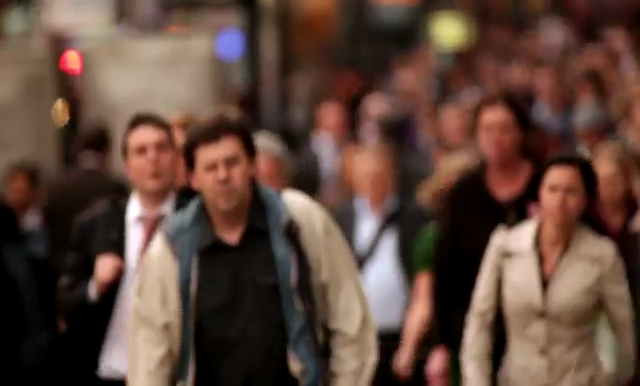
\includegraphics[width=4in]{images/net_benchmarking_screenshot}
		\caption{Screenshot taken from the video used on the benchmark.}
		\label{fig:5_benchmark_screen}
	\end{figure}
	
	
	
	
	\begin{table}[h]
		\centering
		\begin{tabular}{|c|c|c|c|}
			\hline
			\textbf{Architecture} & \textbf{Base network} & \textbf{Dataset} & \textbf{Mean inference time} (ms) \\ \hline
			ResNet  & Inception  & COCO & 820.71 \\ \hline
			SSD  & MobileNet  & COCO & 107.43 \\ \hline
			ResNet  & 101  & COCO & 786.49 \\ \hline
			ResNet  & 50  & COCO & 515.28 \\ \hline
			Inception  & *  & COCO & 349.13 \\ \hline
			ResNet  & 101  & COCO & 63.97 \\ \hline
			Faster-RCNN  & ImageNet  & ILSVRC2014 & 703.99 \\ \hline
			Faster-RCNN  & Inception  & COCO & 352.20 \\ \hline
			ResNet  & 50  & COCO & 793.87 \\ \hline
			*  & MobileNet  & COCO & 106.93 \\ \hline
			SSD  & MobileNet  & COCO & 102.85 \\ \hline
			ResNet  & 101  & COCO & 898.59 \\ \hline
			Inception  & ResNet  & OID & 792.42 \\ \hline
			\textbf{SSD Lite}  & \textbf{MobileNet}  & \textbf{COCO} & \textbf{68.13} \\ \hline
			ResNet  & 101  & Kitti & 111.29 \\ \hline
			Inception  & ResNet  & OID & 667.76 \\ \hline
		\end{tabular}
		\caption{Timing performance tests for several modes. The selected implementation appears in \textbf{boldface}.}
		(*): Not specified.
		\label{tab:5_tests}
	\end{table}
		
	
	
	
	As it can be seen, the vast majority of other implementations (different network architectures) are significantly bigger, which would make impossible to accomplish real-time operation.\\
	
	
	
	
	
	
	
	
	
	